\subsection{债务违约一览}
\begin{frame}{债券违约史}
	债券违约是资本市场中的正常现象
	\begin{itemize}
		\item 2014年,超日债违约打破“刚兑”
		\item 2020年,永煤、华晨违约打破“国企信仰”
		\item 2021年,近期地产债违约大潮
		\item 未来城投债压力
	\end{itemize}
\end{frame}
\begin{frame}{债券违约:分行业}
	\begin{table}[]
		\resizebox{\columnwidth}{!}{%
			\begin{tabular}{llllll}
				\hline
				\multicolumn{1}{c}{\textbf{行业}} & \multicolumn{1}{c}{\textbf{违约债券只数}} & \multicolumn{1}{c}{\textbf{违约债券余额(亿元)}} & \multicolumn{1}{c}{\textbf{余额违约率(\%)}} & \multicolumn{1}{c}{\textbf{违约发行人个数}} & \multicolumn{1}{c}{\textbf{发行人个数违约比率(\%)}} \\ \hline
				信息技术业                        & 36                                        & 423.72                                          & 21.13                                       & 4                                           & 10.00                                               \\
				批发和零售贸易                    & 65                                        & 679.34                                          & 8.93                                        & 15                                          & 9.09                                                \\
				制造业                            & 164                                       & 1,165.98                                        & 8.04                                        & 58                                          & 19.66                                               \\
				农、林、牧、渔业                  & 2                                         & 11.50                                           & 2.63                                        & 2                                           & 9.52                                                \\
				房地产业                          & 27                                        & 267.48                                          & 2.15                                        & 9                                           & 3.57                                                \\
				综合类                            & 75                                        & 705.08                                          & 1.27                                        & 20                                          & 2.55                                                \\
				交通运输、仓储业                  & 34                                        & 350.60                                          & 0.96                                        & 12                                          & 5.08                                                \\
				采掘业                            & 18                                        & 96.11                                           & 0.92                                        & 5                                           & 7.69                                                \\
				建筑业                            & 41                                        & 415.44                                          & 0.61                                        & 11                                          & 0.56                                                \\
				传播与文化产业                    & 1                                         & 3.00                                            & 0.61                                        & 1                                           & 3.70                                                \\
				社会服务业                        & 8                                         & 66.69                                           & 0.39                                        & 6                                           & 1.55                                                \\
				电力、煤气及水的生产和供应业      & 5                                         & 37.98                                           & 0.20                                        & 3                                           & 1.18                                                \\
				金融、保险业                      & 2                                         & 9.99                                            & 0.02                                        & 2                                           & 0.34                                                \\
				\textbf{合计}                     & \textbf{478}                              & \textbf{4,232.91}                               & \textbf{1.45}                               & \textbf{148}                                & \textbf{2.91}                                       \\ \hline
			\end{tabular}
		}
		\caption{违约境内债行业分布\footnote{数据来源:wind}}
		\label{fig:default_indus}
	\end{table}
	如表 \ref{fig:default_indus}所示,违约债券最多的行业是制造业,其次是综合类、批发和零售贸易。近期热点的主要是房地产类,2021年来实质违约、展期的房地产企业包括但不限于重庆协信、华夏幸福、四川蓝光、花样年、新力控股、当代置业、鑫苑置业、中国奥园、阳光城、佳兆业、恒大、阳光100等
\end{frame}

\begin{frame}{违约债:分地域}
	\begin{columns}
		\column{0.6\linewidth}
		\begin{figure}
			\centering
			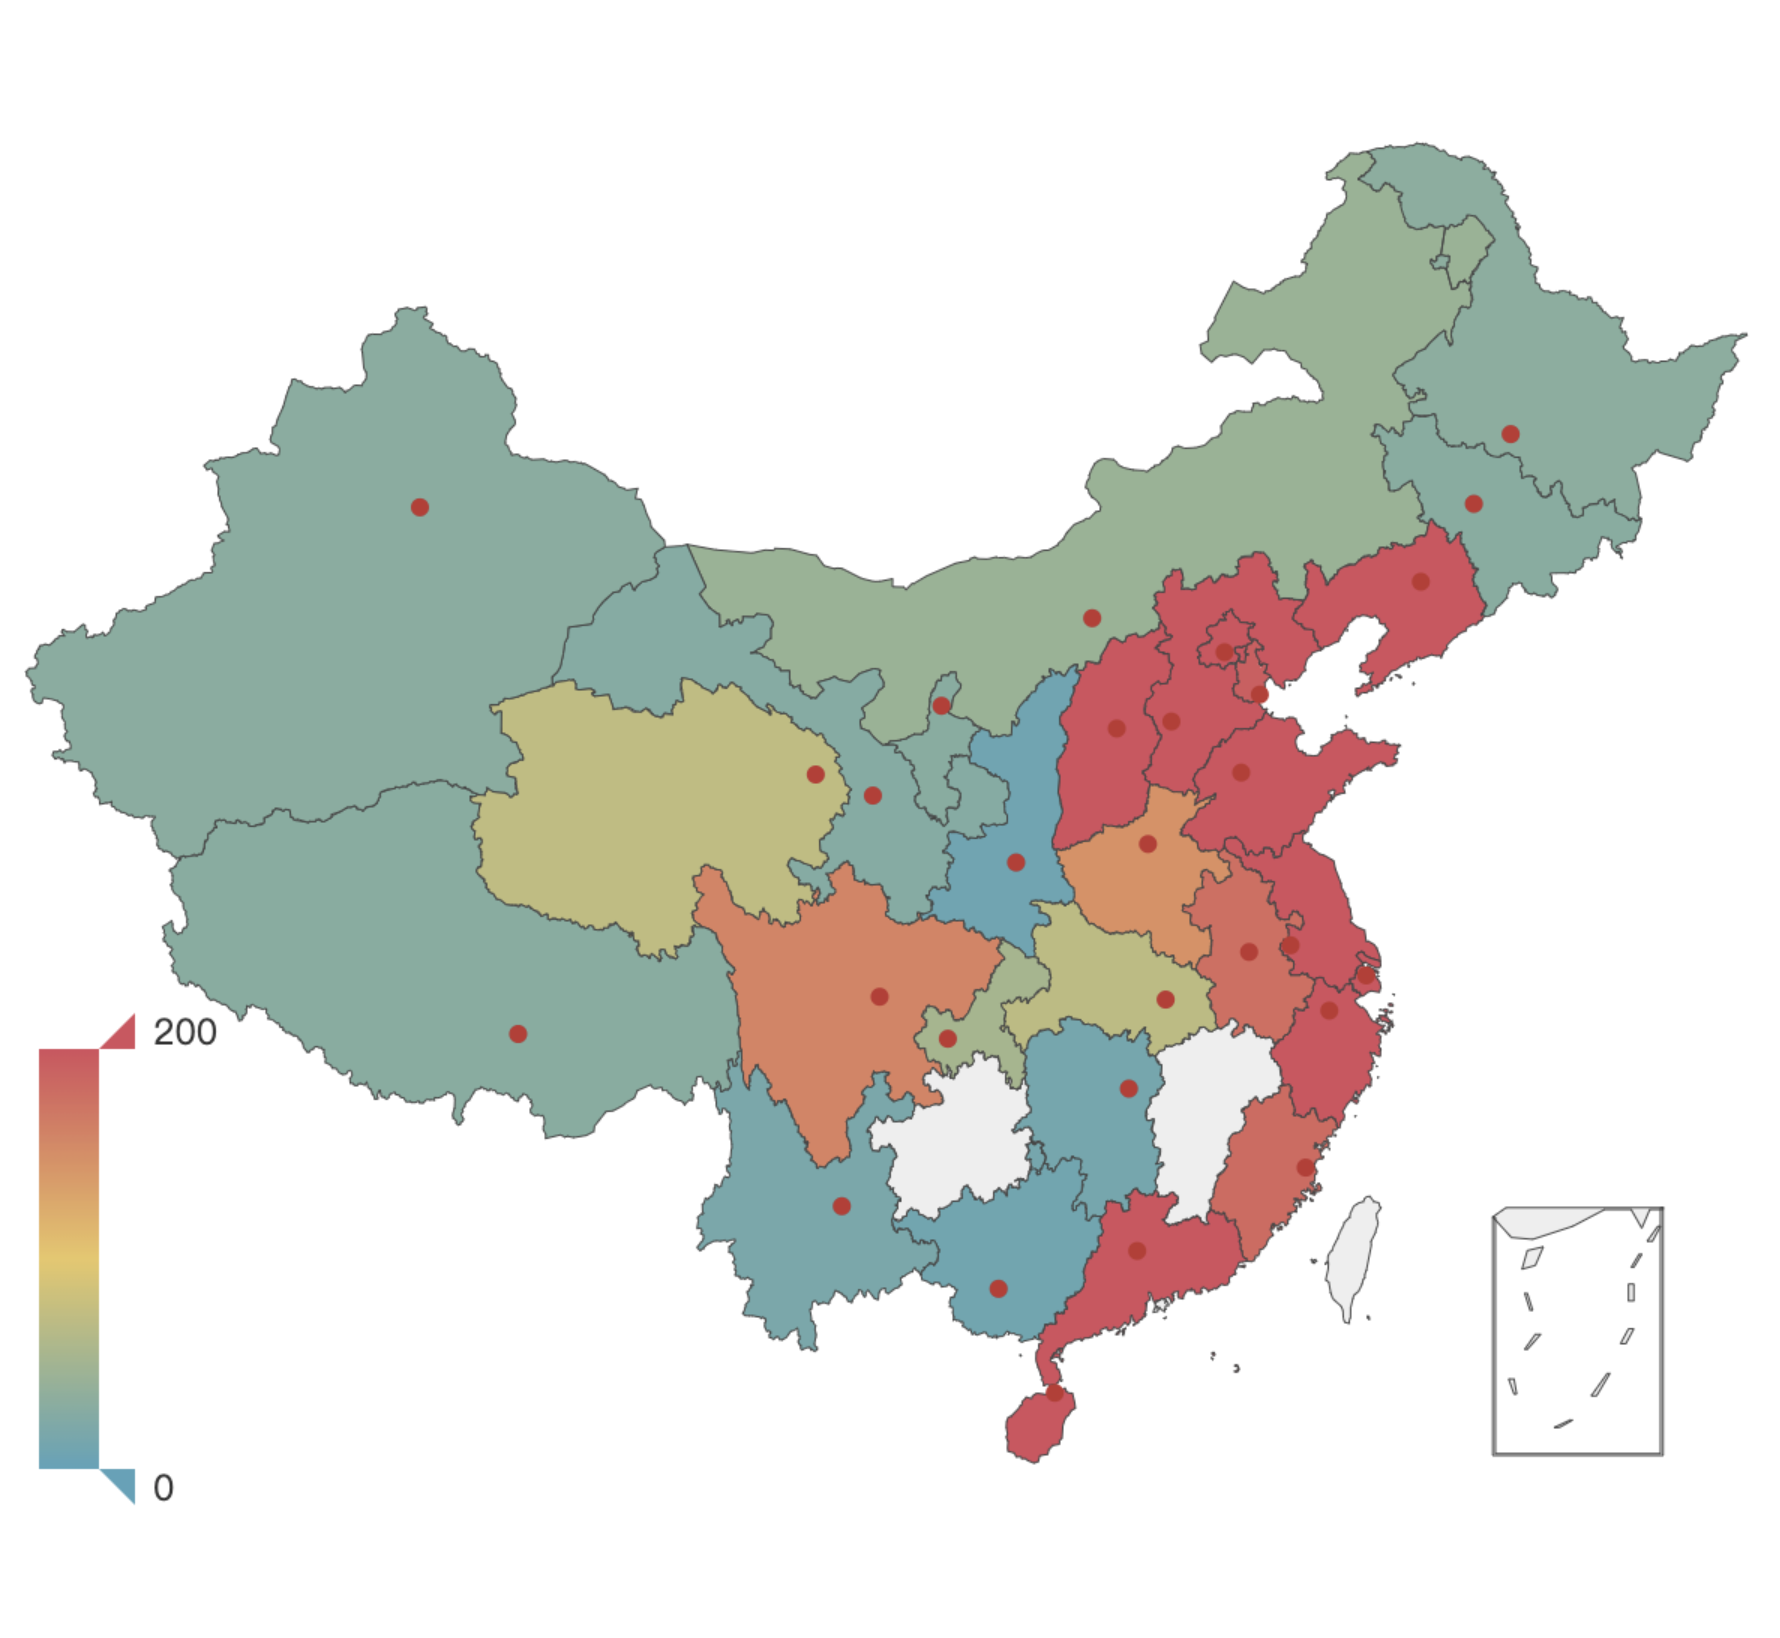
\includegraphics[width=\linewidth]{lib/default_by_geo.png}
			\caption{违约债券余额}
			\label{fig:defaultGeo}
		\end{figure}
		\column{0.35\linewidth}
		北京以违约债券105只、1,212.40亿元占第一位。

		一方面经济落后地区违约风险较大,一方面经济较好的地区企业发债数量较多可能导致违约金额较大,图\ref{fig:defaultGeo}显示出后一种作用较强。
	\end{columns}
\end{frame}
\subsection{债务违约后果}
\begin{frame}{对持有人}
	\begin{columns}[c]
		\column{0.4\linewidth}
		对于债券人持有人而言,不仅面临债券违约带来的本金损失,还将引发一系列问题。
		\begin{itemize}
			\item 机构面临赎回带来的流动性压力
			\item 结构化发行,或引发交易纠纷
			\item 投入较长的求偿时间,清偿率平均越20\%
		\end{itemize}
		\column{0.5\linewidth}
		\begin{figure}
			\centering
			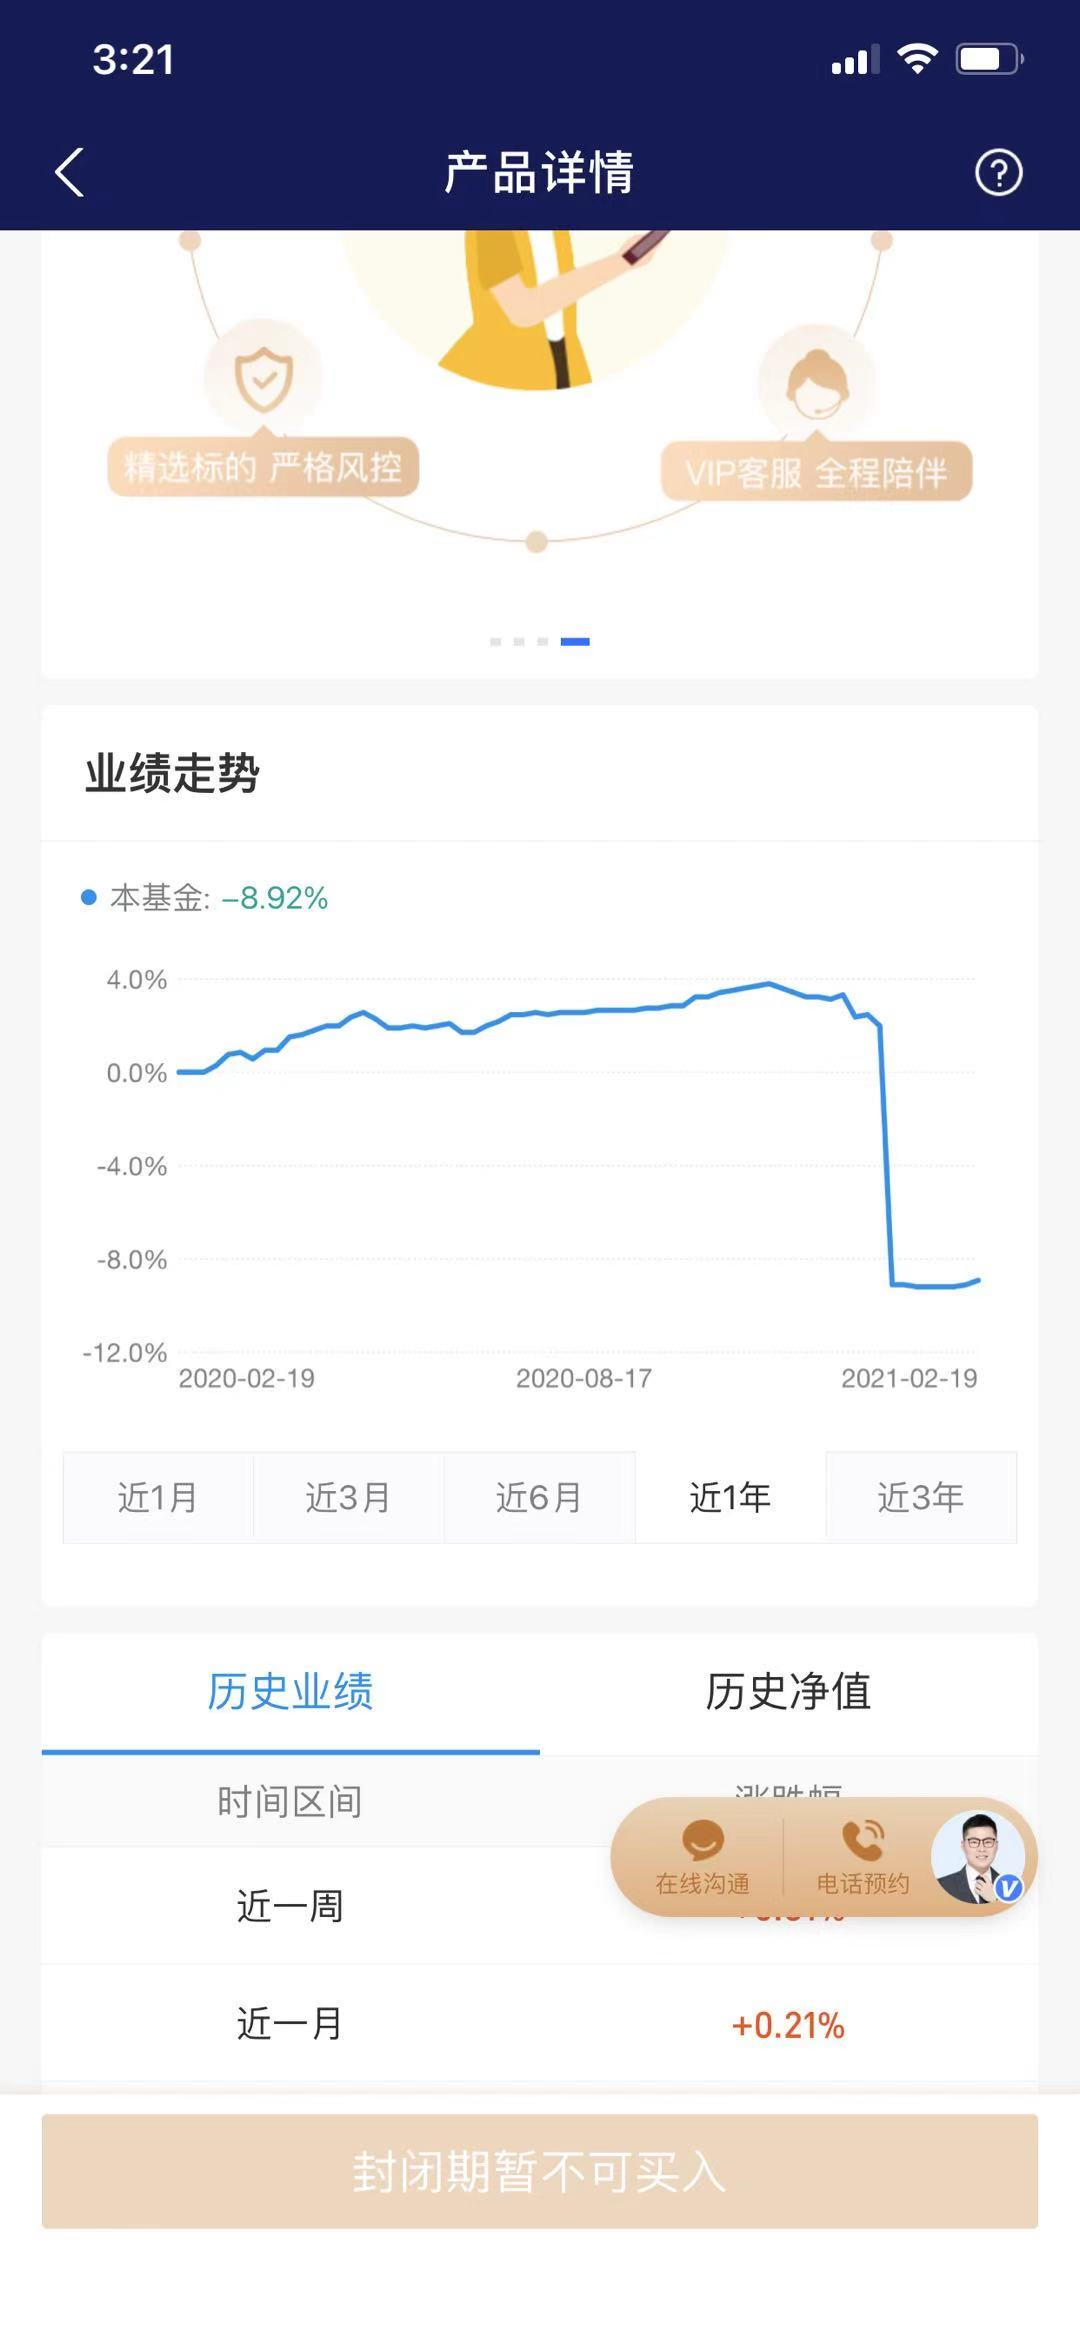
\includegraphics[width=0.6\linewidth]{lib/jsfund.jpg}
		\end{figure}
	\end{columns}
\end{frame}
\begin{frame}{对发行人}
	\begin{itemize}
		\item 削弱外部融资功能
		\item 交叉违约条款引发偿债压力急升
		\item 负面事件引发内部管理层动荡
		\item 影响企业的生产经营
	\end{itemize}
\end{frame}
\begin{frame}{外部性}
	\begin{columns}[c]
		\column{0.5\linewidth}
		企业信用风险可能会传染,可能是由于股权、业务/地区相似或投资人心理,引发进一步的危机。\newline
		2020年11月10日,永煤违约之后,一级市场上河南方面拟发行的5只债券没有一只发行成功,一个月内累计1000亿信用债取消发行;二级市场上清控、豫能化债券价格闪崩,并最终违约。
		\column{0.5\linewidth}
		\begin{figure}
			\centering
			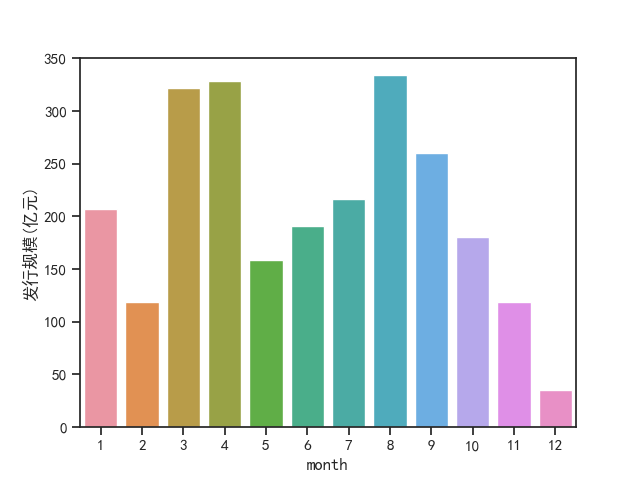
\includegraphics[width=\linewidth]{lib/henan.png}
			\caption{国企信仰崩塌,河南信用债发行骤减}
		\end{figure}
	\end{columns}
\end{frame}
